\usetikzlibrary{trees,shadows}
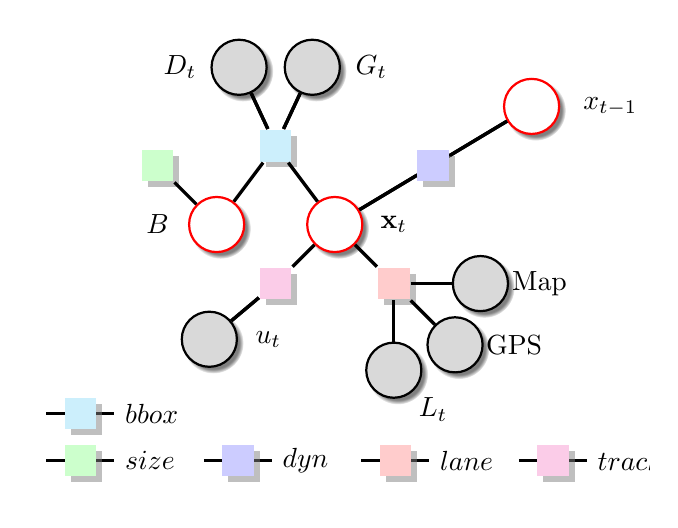
\begin{tikzpicture}[grow cyclic, line width=1.2pt,
    variablenode/.style={circle,circular drop shadow,draw=red,fill=white,thick,minimum width=0.7cm},
    factor/.style={rectangle,drop shadow,fill=white,thick,minimum width=1.2cm},
    factor1/.style={rectangle,drop shadow,fill=green!20  ,thick,minimum width=0.4cm,minimum height=0.4cm},
    factor2/.style={rectangle,drop shadow,fill=blue!20   ,thick,minimum width=0.4cm,minimum height=0.4cm},
    factor3/.style={rectangle,drop shadow,fill=red!20    ,thick,minimum width=0.4cm,minimum height=0.4cm},
    factor4/.style={rectangle,drop shadow,fill=cyan!20   ,thick,minimum width=0.4cm,minimum height=0.4cm},
    factor5/.style={rectangle,drop shadow,fill=magenta!20,thick,minimum width=0.4cm,minimum height=0.4cm},
    level distance=1.10cm,
  obs/.style={fill=gray!30,draw=black},
  prevf/.style={draw=green!20,text=gray},
  prevobsv/.style={draw=gray!10,fill=gray!1,text=gray},
  prevv/.style={draw=red!20,text=gray}
]
  \path[use as bounding box,clip] (-4.9, -3.5) rectangle (3,2.5);


  \path
  (-2.5,0) node[variablenode](dim) {}
  +(-0.75, 0) node {$B$}
  +(-0.75,0.75) node[factor1](fsize){}
  ;

  \begin{scope}[line width=0.5pt]
    \path 
    % t-1 layer
    (1.5,1.5) node [variablenode] (xt1) {}
    +(1.0, 0) node {$x_{t-1}$}
  %  [counterclockwise from=-100,sibling angle=60]
  %  +(1.0, -1.0) node [factor,prevf] (flane1) {$E_{lane}$} 
  %  child { node [variablenode,obs,prevobsv] (l1) { $L_t$ } }
  %  child { node [ variablenode,obs,font=\footnotesize,prevobsv] (gps1) {GPS}}
  %  child { node [ variablenode,obs,font=\footnotesize,prevobsv] (map1) {Map}}

  %  [counterclockwise from=220]
  %  +(-1.0, -1.0) node[factor,prevf](fpt1) {$E_{pt}$}
  %  child { node[variablenode,obs,prevobsv](pt1){$u_t$} }

  %  [counterclockwise from=60,sibling angle=60]
  %  +(-1, 1.0) node[factor,prevf](fdet1){$E_{det}$} 
  %   child {
  %     node[variablenode,obs,prevobsv](gp1){$G_t$} 
  %   }
  %   child { node[variablenode,obs,prevobsv](Det1){$D_t$}
  %   }

    ;

  %\draw [gray](xt1) -- (fdet1) -- (dim);
  %\draw [gray](xt1) -- (flane1);
  %\draw [gray](xt1) -- (fpt1);
      
  \end{scope}

   %(0.5,1.0) node [factor2] (fdynx) {}
  %(1.95,1.8) node [factor,draw=gray,text=gray,minimum width=1cm] (fdynt) {$E_{d}$}

 %(0.2,2.0) node[factor](fhol) {$E_{hol}$}

  %(1, 0)  node[variablenode](theta){$\theta_t$}
  \path
  [counterclockwise from=-90,sibling angle=45]
  (-1, 0)  node[variablenode](xt) {}
  + (0.75, 0) node {$\mathbf{x}_t$}
  + (0.75, -0.75) node [factor3] (flane) {} 
  child { node [variablenode,obs] (l) {} +(.5,-0.5) node { $L_t$ } }
  child { node [ variablenode,obs,font=\footnotesize] (gps) {} +(.75,0) node {GPS}}
  child { node [ variablenode,obs,font=\footnotesize] (map) {} +(.75,0) node {Map}}

  [counterclockwise from=65,sibling angle=50]
  (-1.75, 1.0) node[factor4](fdet){} 
  child {
    node[variablenode,obs](gp){} +(.75,0) node {$G_t$} 
  }
  child {           node[variablenode,obs](Det){} +(-.75,0) node {$D_t$}
  }

  [counterclockwise from=220]
  (-1.75, -0.75) node[factor5](fpt) {}
  child { node[variablenode,obs](pt){} +(.75,0) node {$u_t$} }
  ;
  \draw (xt) edge node [factor2] (fdynx) {} (xt1);
  \draw (xt) -- (fdet) -- (Det);
  \draw (xt) edge (fpt);
  \draw (fpt) -- (pt);
  %\path  (fpt) edge (theta);
  \draw (fdet) -- (gp);
 %(0.2,2.0) node[factor](fhol) {$E_{hol}$}
  %\draw (xt) edge [bend left=40] node[factor] (fhol) {$E_{hol}$} (xt1);
  %\draw (fhol) -- (theta);  	  
  \draw (dim) -- (fdet);
  \draw (fsize) -- (dim);
  %\draw (theta) -- (flane);
  \draw (xt) -- (fdynx) -- (xt1);
  %\draw (theta) -- (fdynt) -- (theta1);
  \draw (xt) -- (flane);

  % Legend
  \path (-4.8, -3.0) node (ls) {}
  ++(1.0, 0) node [anchor=west] (e1e) {$\Energy{size}$}
  ++(1.0, 0) node [] (e2s) {}
  ++(1.0, 0) node [anchor=west] (e2e) {$\Energy{dyn}$}
  ++(1.0, 0) node [] (e3s) {}
  ++(1.0, 0) node [anchor=west] (e3e) {$\Energy{lane}$}
  ++(1.0, 0) node [] (e5s) {}
  ++(1.0, 0) node [anchor=west] (e5e) {$\Energy{track}$};
  \path (ls)
  ++(0, 0.60) node [] (e4s) {}
  ++(1.0, 0) node [anchor=west] (e4e) {$\Energy{bbox}$};
  ;
  \draw (ls) edge node [factor1] {} (e1e) ;
  \draw (e2s) edge node [factor2] {} (e2e) ;
  \draw (e3s) edge node [factor3] {} (e3e) ;
  \draw (e4s) edge node [factor4] {} (e4e) ;
  \draw (e5s) edge node [factor5] {} (e5e) ;
\end{tikzpicture}
